%\documentclass[a4paper]{article}
\documentclass[a4paper,fleqn,12pt]{JMThesis}
%%% These are PDF packages needed to include PDF pictures
\usepackage[pdftex]{graphicx}
\DeclareGraphicsExtensions{.pdf}


\usepackage[OT2,T1]{fontenc}
\usepackage[english,serbian]{babel}

\newcommand{\cyr}{\fontencoding{OT2}\selectfont\selectlanguage{serbian}}
\newcommand{\latin}{\fontencoding{T1}\selectfont\selectlanguage{english}}

\usepackage{cmsrb}
% \usepackage[serbian]{babel}
\usepackage[utf8]{inputenc}

% \usepackage[OT2]{fontenc}
% \newcommand{\latin}{\fontencoding{T1}\selectfont}
\usepackage{substitutefont}

\renewcommand{\ch}{\v c}
\newcommand{\Ch}{\v C}
\renewcommand{\sh}{\v s}
\newcommand{\Sh}{\v S}
\newcommand{\zh}{\v z}
\newcommand{\Zh}{\v Z}

\renewcommand{\baselinestretch}{1}
\usepackage{amsfonts}
\usepackage{amssymb}
\usepackage{amsthm}
\usepackage{amsmath}
%\usepackage{gclc}
\usepackage{newlfont}
\usepackage{graphicx}
\usepackage{color}
\usepackage{verbatim,enumerate}
\usepackage{wasysym}
\usepackage{mdwlist}
\usepackage{multicol}
\usepackage{fancyhdr}
\usepackage{tocloft}
\usepackage[
backend=biber,
style=apa,
sorting=ynt
]{biblatex}
\DeclareLanguageMapping{serbian}{serbian-apa}

\usepackage[font=small,labelfont=bf]{caption}

\counterwithout{figure}{chapter}
\newcommand\DS{\displaystyle}
\newcommand\TS{\textstyle}
\newcommand{\konj}[1]{\overline {\rule {0pt}{7pt}{#1}}\,}
\oddsidemargin 1cm

\evensidemargin 0cm

\textwidth 15cm

\definecolor{Light}{gray}{.80}
\definecolor{Dark}{gray}{.20}

\pagestyle{headings}

\theoremstyle{plain}

\theoremstyle{definition}

 \newtheorem{pr}{Primer}
 \newtheorem{te}{Teorema}[chapter]
 \newtheorem{teo}{Teorema}[chapter]
 \newtheorem{lem}{Lema}[chapter]
 \newtheorem{lema}{Lema}[chapter]
 \newtheorem{po}{Posledica}
 \newtheorem{de}{Definicija}[chapter]
 \newtheorem{za}{Zadatak}
 \newtheorem{reza}{Reshenje}
 \newtheorem{fm}{F}

\newcommand{\dok}{\noindent \textit{Dokaz:}}

\newcommand{\zbn}{\sum_n}
\newcommand{\zbng}{\sum_{n=0}^\infty}
\newcommand{\zbk}{\sum_k}
\newcommand{\zbkg}{\sum_{k=0}^\infty}
\newcommand{\zbi}{\sum_i}
\newcommand{\zbig}{\sum_{i=0}^\infty}
\newcommand{\zbj}{\sum_j}
\newcommand{\zbjg}{\sum_{j=0}^\infty}
\newcommand{\zbtg}{\sum_{t=0}^\infty}
\newcommand{\osr}{\,_{\,\leftrightarrow}^{osr}\,}
\newcommand{\esr}{\,_{\,\leftrightarrow}^{esr}\,}
\newcommand{\piopt}{{\pi}^{*}}
\DeclareMathOperator{\EX}{\mathbb{E}}% expected value

\renewcommand*{\proofname}{Dokaz}
%\renewcommand*{\refname}{Literatura}
%\renewcommand{\figurename}{Slika.$ $ }
\theoremstyle{definition}

% Donji i gornji navosnici
\def\zn{,\kern-0.09em,}
\def\zng{'\kern-0.09em'}
\pagenumbering{roman}
\addbibresource{references.bib}

\begin{document}
% \thispagestyle{empty}
% \textcolor{white}{proba}
% \clearpage

\thispagestyle{empty}

\begin{center}
{\LARGE Ra\ch unarska gimnazija}
\end{center}
\vspace*{50mm}

\begin{center}
{\huge МАТУРСКИ РАД}

\vspace*{8pt}
{\Large Napredne tehnike programiranja}
\end{center}

\vspace*{10pt}
\begin{center}
{\LARGE Primena u\ch enja sa podsticajem za re\sh avanje Atari igara}
\end{center}

\vspace*{70mm}
\setlength{\columnsep}{50pt}
\begin{multicols}{2}
 {\noindent \Large Autor:
\\Ognjen Ne\sh ković}


{ \noindent \hfill \Large Mentor:\\
\hfill \phantom{aaaaaaaa}  dr Filip Marić}
\end{multicols}

\vfill
\begin{center}
{\Large Beograd, maj 2022.}
\end{center}

\newpage

\renewcommand{\contentsname}{Sadr\zh aj}
\thispagestyle{empty}
\pagenumbering{gobble}
\tableofcontents \clearpage

\pagenumbering{arabic}
\renewcommand{\chaptername}{}
\setcounter{page}{1}
\thispagestyle{plain}
{\Large Sa\zh etak}\\ 
Lorem ipsum dolor sit amet, consectetur adipiscing elit.

\chapter[Uvod]{Uvod}
\thispagestyle{plain}
\section[Osnove]{Osnove}
Još od davnina ljudi su se nadmetali u igranju igara poput šaha, 
kineske igre {\latin Go}, {\latin Backgammon} itd. 
U mnogim kulturama oni koji su bili najbolji u ovim igrama 
bili su izuzetno poštovani, pa bi neki ljudi posvećivali čak i 
čitav svoj život usavršavanju svoje strategije u nekoj od ovih 
igara. Stoga, dugo se smatralo da je sposobnost igranja ovih igara 
nešto jedinstveno za ljude i da je stvaranje mašine ili algoritma 
sposobnog da pobedi najboljeg šahistu ili drugog profesionalnog 
igrača gotovo nemoguće. \\
Ovaj izazov mučio je matematičare stotinama godina i ostao je 
neprevaziđen sve do 1997. godine kada je konačno računar 
{\latin (Deep blue)} prvi put pobedio najboljeg šahistu tog 
vremena Garija Kasparova {\latin (\cite{campbell2002deep})}. 
{\latin Deep blue} je koristio alfa-beta algoritam pretrage, 
heuristike, ekspertsko znanje i specijalni hardver napravljen 
kako bi probao što veći broj poteza po sekundi. 
Postojao je veći broj šahovskih mašina koje su prethodile 
{\latin Deep blue} mašini. Kako bi se razvio {\latin Deep blue} 
bilo je potrebno puno šahista, programera, vremena i novca. 
Dakle, jasno je da iako su velik uspeh, {\latin Deep blue} 
i njemu slične mašine nisu veoma generalne ili uopšte primenljive 
van vrlo specijalizovanog domena za koji su napravljene.\\
Velika prekretnica došla je sa razvojem neuronskih mreža, 
učenja sa podsticajem i hardvera. Sve ovo omogućilo je da se 
razviju generalni algoritmi koji bez velike modifikacije mogu 
naučiti da veoma dobro igraju veliki broj igara {\latin (\cite{mnih2015human})}. 
Sledeći veliki korak u mašinskom igranju igara došao je sa 
programom {\latin Alpha Go} koji je 2016. godine pobedio 
svetskog šampiona Li Sedola u igri Go. {\latin Alpha Go} je 
koristio učenje sa podsticajem, konvolucione neuronske mreže, 
Monte Karlo pretragu, takođe delimično je bio treniran na igrama 
koje su igrali profesionalni Go igrači {\latin (\cite{silver2017mastering})}. 
Godinu dana kasnije - 2017. godine objavljena je verzija {\latin Alpha Go-a} 
koja ne koristi ikakvo ekspertsko znanje - {\latin Alpha Go Zero}, 
koja postiže čak bolji rezultat od verzije trenirane sa ekspertskim 
igrama. Poslednji veliki napredak je program {\latin AlphaStar} 
koji igra stratešku video igru {\latin StarCraft II} gde pobeđuje 
najbolje igrače ove igre {\latin (\cite{vinyals2019grandmaster})}.\\
Glavna razlika između metoda korišćenih za rešavanje šaha 
(alfa-beta pretraga) i savremenih metoda je način kako se 
igra modeluje. U savremenim metodama učenja sa podsticajem 
problemi koje je potrebno rešiti predstavljaju se kao Markovljevi 
procesi odlučivanja. Ako se problem ovako prestavi u nekim 
jednostavnim slučajevima se može rešiti dinamičkim programiranjem, 
a za složenije slučajeve se rešenje može aproksimirati neuronskim 
mrežama.

\section[Motivacija]{Motivacija}
Igre ili opštije, problemi koji se mogu predstaviti kao Markovljevi procesi odlučivanja su od velikog teoretskog značaja za mašinsko učenje. Pored toga što donekle pružaju uvid u mogućnosti računara i razlike između ljudske i veštačke inteligencije, veliki broj procesa u stvarnosti poput problema optimalne kontrole (upravljanje robotima i mašinama), regulisanje sistema za hlađenje, kompresije videa itd. mogu se modelovati kao Markovljevi procesi odlučivanja. Složene igre pružaju dobar način da se granice savremenih metoda preciznije odrede, što primenu onda čini znatno lakšom. 
\section [Cilj Rada]{Cilj rada}
Cilj ovog rada je da se izlože metode učenja sa podsticajem od najjednostavnijih do složenijih. Uz ovo prikazani su problemi koji su rešivi svakom od metoda i problemi koji prevazilaze mogućnosti date metode, pa motivišu upotrebu neke složenije metode.

\chapter[Metode]{Metode}
\section[Uvod]{Uvod}
U narednom delu će biti razmatrane varijante Markovljevog procesa odlučivanja i rešenja koja su moguća za te varijante, pa je potrebno definisati Markovljev proces odlučivanja i uvesti potrebnu notaciju.
Markovljevi procesi odlučivanja su uopštenje Markovljevih lanaca sa dodatim akcijama, za definiciju markovljevog procesa potrebno je difinisati sledeće:
\begin{itemize}
	\item Skup stanja $S$
 	\item Skup akcija $A$ i $A_s$ - skup mogućih akcija u stanju $s$
	\item $P_a(s,s') = P(s_{t+1} = s' \mid s_t = s, a_t = a)$  - verovatnoću da se završi u stanju $s'$ ako je u stanju $s$ izvršena akcija $a$
	\item $R_a(s,s')$ - nagrada koja se ostvaruje kada se u stanju $s$ izvrši akcija $a$ i završi u stanju $s'$
 	\item Funkcija (politika) $\pi(s) : S \rightarrow A$ koja predstavlja igrača (onog koji donosi odluku), pa za dato stanje $s$ iz skupa stanja $S$ određuje akciju koju treba izvršiti 
\end{itemize}
Rešenje Markovljevog procesa odlučivanja je optimalna funkcija $\piopt$:
\[
	\text{\latin argmax}_{\piopt}\EX \left[ \zbtg \gamma^t R_{\piopt(s_t)}(s_t,s_{t+1}) \right]
\]
Posmatrajmo jednostavan Markovljev proces odlučivanja sa tri stanja ${S_0, S_1, S_2}$ i dve moguće akcije ${A_0, A_1}$ (slika 1).
\begin{figure}[!ht]
	\centering
	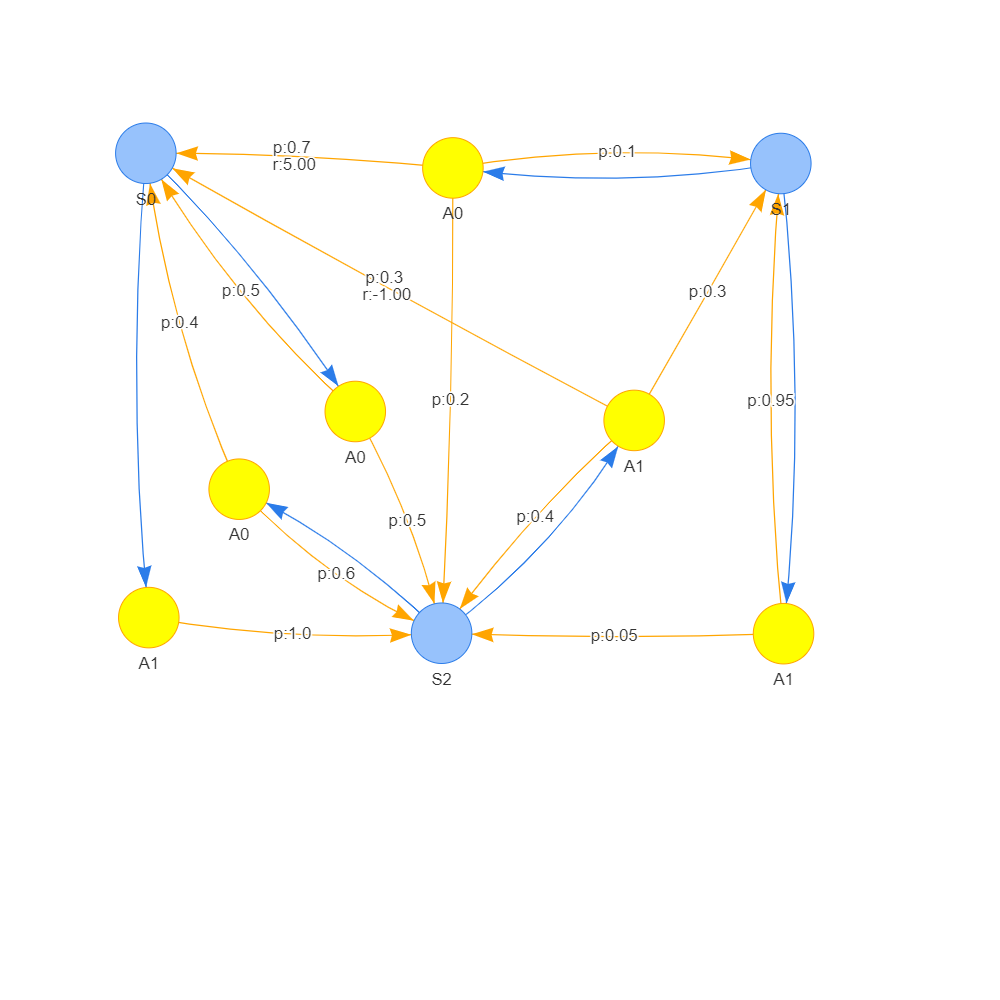
\includegraphics[scale=0.4]{../graph-visuals/example-mdp.png}
	\caption{Primer Markovljevog procesa odlučivanja}
\end{figure}

Primetimo da ukoliko se fiksira neka politika $\pi$, na primer $\pi(S_0)=A_0, \pi(S_1)=A_0, \pi(S_2)=A_1$ proces sa slike 1 postaje ekvivalentan novom procesu (slika 2).
\begin{figure}[!ht]
	\centering
	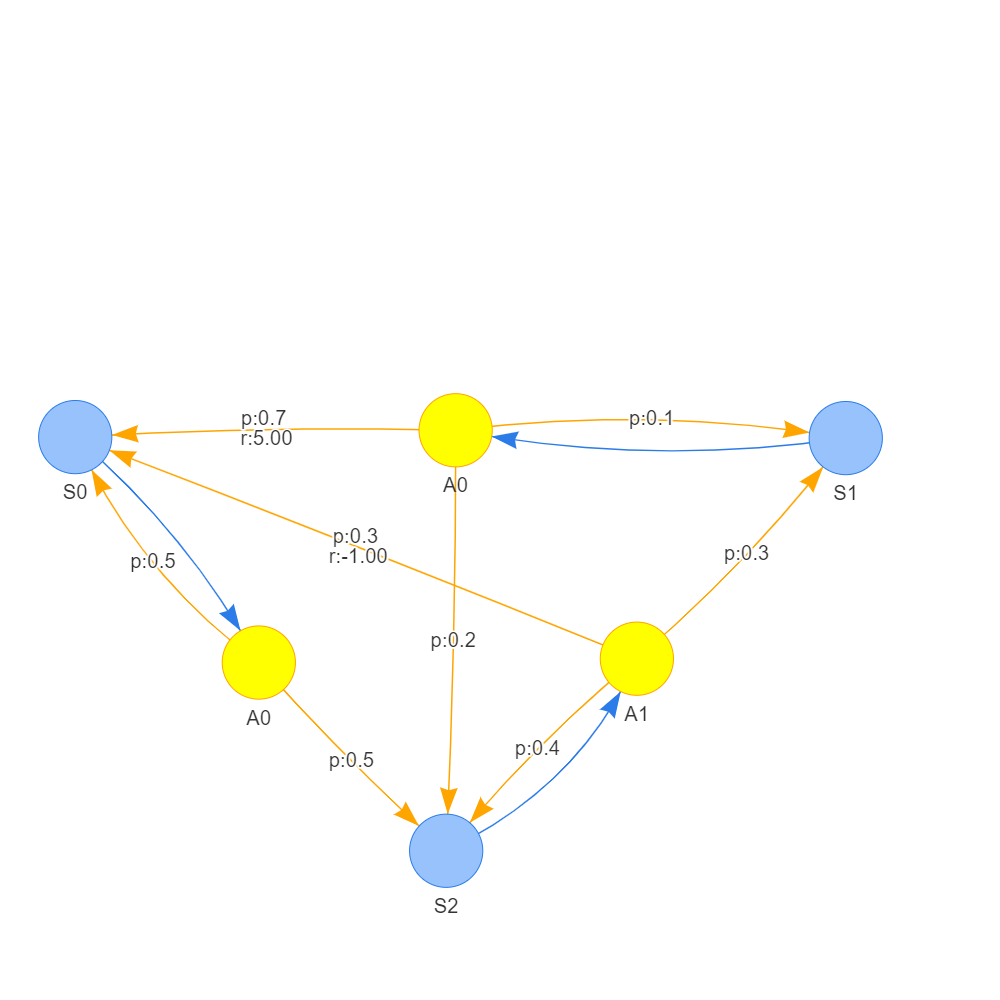
\includegraphics[scale=0.4]{../graph-visuals/example-mdp-given-policy.png}
	\caption{Markovljev proces pod politikom $\pi$}
\end{figure}

Dodatno, lako je videti da je tako dobijen proces (slika 2) ekvivalentan sledećem Markovljevom lancu, sa dodatim nagradama (slika 3).
\begin{figure}[!ht]
	\centering
	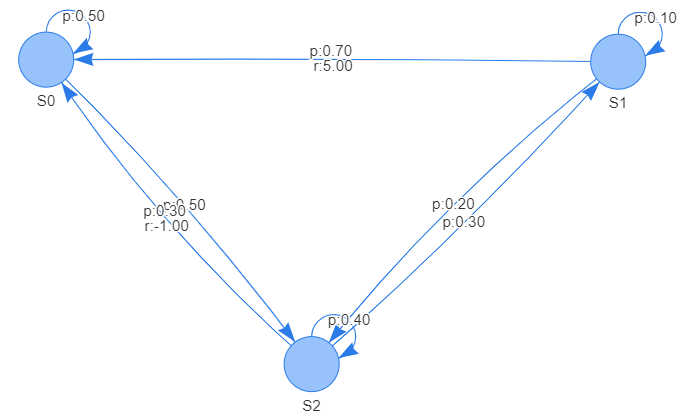
\includegraphics[scale=0.4]{../graph-visuals/example-mdp-given-policy-chain.png}
	\caption{Ekvivalentan Markovljev lanac sa nagradama}
\end{figure}
Kada je dat ovakav lanac, kao sa slike 3, postavlja se pitanje: kako efikasno odredti očekivanu nagradu u tonm lancu, ako je dato početno stanje ili verovatnoće da svako stanje bude početno. Ako je ovo moguće uraditi, onda je odmah dat efikasan način da se evaluira očekivana nagrada koja će biti ostvarena ako se koristi neka fiksna politika.\\

\section{Evaluacija politike ({\latin policy evaluation})}
Kada je politika fiksirana, traženje očekivane nagrade koja će biti ostvarena ako se prati data politika je ekvivalentna nalaženju očekivane nagrade u nekom markovljevom lancu. Prvo, uvedimo sledeću notaciju:
\begin{itemize}
	\item $S_t$ - Skup svih sekvenci dužine $t$. Na primer ako se iz stanja $N_0$ poseti stanje $N_1$, pa stanje $N_2$ itd. pa se na kraju poseti stanje $N_t$ sekvenca bi bila $(N_0, N_1, N_2, \cdots , N_t)$
 	\item $S_{t,u}$ - Skup svih sekvenci stanja dužine $t$ koje se završavaju sa stanjem $u$.
  	\item $T(u,v)$ - Verovatnoća da se iz stanja $u$ pređe u stanje $v$.
   	\item $p(s), s \in S_t$ - Verovatnoća da se neka sekvenca dogodi. Ako je data sekvenca $s=(N_0,N_1,N_2,\cdots , N_t)$ onda je $p(s) = T(N_0, N_1)\cdot T(N_1,N_2)\cdots T(N_{t-1},N_{t})$
    \item $R(u,v)$ - Nagrada kada se iz stanja $u$ završi u stanju $v$.
    \item $r(s), s \in S_t$ - Nagrada za datu sekvencu $s$. 
    \[ 
		\begin{split}
		r(s) &= R(N_0, N_1)+\gamma R(N_1,N_2) +\gamma^2 R(N_2,N_3) \cdots + \gamma^{t-1} R(N_{t-2},N_{t-1}) \\
		\gamma &< 1
		\end{split}
	\]
    \item $L(u,t)$ - Verovatnoća da se posle $t$ koraka završi u stanju $u$. 
	\[ 
		L(u,t) = \sum_{s \in S_{t,u}}p(s)
	\]
    \item $E_r(t)$ - Očekivana nagrada posle t koraka.
    \[
		E_r(t) = \sum_{s \in S_t}p(s)r(s)
	\]
\end{itemize}
\lem $L(u,t) = \sum_{v}T(v,u)L(v,t-1)$
\[
\begin{split}
	L(u,t) &= \sum_{s \in S_{t,u}}p(s)	\\
	L(u,t) &= \sum_{N_0, N_1, \cdots, N_{t-1}}T(N_0,N_1)\cdot T(N_1,N_2)\cdots T(N_{t-2},N_{t-1})\cdot T(N_{t-1},u)\\
	L(u,t) &= \sum_{v}\sum_{N_0, N_1,\cdots , N_{t-2}}T(N_0,N_1)\cdot T(N_1,N_2)\cdots T(N_{t-2},v) \cdot T(v,u)\\
	L(u,t) &= \sum_{v}T(v,u)\sum_{N_0, N_1,\cdots , N_{t-2}}T(N_0,N_1)\cdot T(N_1,N_2)\cdots T(N_{t-2},v)\\
	L(u,t) &= \sum_{v}T(v,u)L(v,t-1)
\end{split}
\]
Ako definišemo da je $L(t)$ vektorska funkcija, a $T$ matrica možemo prethodnu jednačinu zapisati elegantnije kao:
\[ L(t) = L(t-1)T \]
Kako je $L(0) = L_0$ gde je $L_0$ Verovatnoća da se počne iz svakog stanja. Lako se može pokazati da je:
\[ L(t) = L_0T^t \]
\lem $E_r(t) = E_r(t-1) + \gamma^{t-1}\sum_{u}\sum_{v}T(u,v)R(u,v)L(u,t)$
\[
\begin{split}
	E_r(t) &= \sum_{s \in S_t}p(s)r(s)	\\
	E_r(t) &= \sum_u \sum_{s' \in S_{t-1,u}}p(s')\sum_{v}T(u,v)(R(s') + \gamma^{t-1} R(u,v))\\
	E_r(t) &= \sum_u \sum_{s' \in S_{t-1,u}}p(s')(\sum_{v}T(u,v)R(s') + \gamma^{t-1} \sum_{v}T(u,v)R(u,v))\\
	E_r(t) &= \sum_u \sum_{s' \in S_{t-1,u}}p(s')(R(s')\sum_{v}T(u,v) + \gamma^{t-1} \sum_{v}T(u,v)R(u,v))\\
	E_r(t) &= \sum_u \sum_{s' \in S_{t-1,u}}p(s')(R(s')\cdot 1 + \gamma^{t-1} \sum_{v}T(u,v)R(u,v))\\
	E_r(t) &= \sum_u \sum_{s' \in S_{t-1,u}}p(s')(R(s') + \gamma^{t-1} \sum_{v}T(u,v)R(u,v))\\
	E_r(t) &= \sum_u \sum_{s' \in S_{t-1,u}}\left(p(s')R(s') + p(s')\gamma^{t-1}\sum_{v}T(u,v)R(u,v)\right)\\
	E_r(t) &= \sum_u \sum_{s' \in S_{t-1,u}}p(s')R(s') + \gamma^{t-1}\sum_u \sum_{s' \in S_{t-1,u}}p(s')\sum_{v}T(u,v)R(u,v)\\
	E_r(t) &= \sum_{s' \in S_{t-1}}p(s')R(s') + \gamma^{t-1}\sum_u \sum_{s' \in S_{t-1,u}}p(s')\sum_{v}T(u,v)R(u,v)\\
	E_r(t) &= E_r(t-1) + \gamma^{t-1}\sum_u \sum_{s' \in S_{t-1,u}}p(s')\sum_{v}T(u,v)R(u,v)\\
	E_r(t) &= E_r(t-1) + \gamma^{t-1}\sum_u \left(\sum_{v}T(u,v)R(u,v) \cdot \sum_{s' \in S_{t-1,u}}p(s')\right)\\
	E_r(t) &= E_r(t-1) + \gamma^{t-1}\sum_u \sum_{v}T(u,v)R(u,v) \cdot L(u,t)\\
\end{split}
\]
Dodatno možemo primetiti sledeće:
\[
	\sum_u \sum_{v}T(u,v)R(u,v) \cdot L(u,t) = \sum_u L(u,t)\sum_{v}T(u,v)R(u,v)
\]
Ukoliko definišemo $L(t)$ kao vektorsku funkciju, tako da je $L(t)_u$ verovatnoća da se u trenutku $t$ bude u stanju $u$ i primetimo da je $\sum_{v}T(u,v)R(u,v)$ konstantan vektor $\vec{c}$.
Možemo zapisati izraz kao:
\[
	E_r(t) = E_r(t-1) + \gamma^{t-1}\vec{L(t)} \cdot \vec{c}
\]  
Pa je lako videti da je:
\[
	\begin{split}
	E_r(t) &= \sum_{i=1}^{t}\gamma^{i-1}\vec{L(i)} \cdot \vec{c}\\
	E_r(t) &= \vec{c} \cdot \sum_{i=1}^{t}\gamma^{i-1}\vec{L(i)}
	\end{split}
\]
\medskip
Za aciklične markovljeve lance, odnosno za aperiodične matrice $T$ izračunavanje $E_r(t)$ za dovoljno veliko $t$ je dovoljno za nalaženje očekivane nagrade.
Međutim za periodične matrice $T$ je potrebno pokazati da $\lim_{t \to \infty}{E_r(t)}$ postoji.
\lem $\lim_{t \to \infty}{E_r(t)} = \text{const}$\\
Ako se u izraz $E_r(t) = \vec{c} \cdot \sum_{i=1}^{t}\gamma^{i-1}\vec{L(i-1)}$ zameni definicija za $\vec{L(i)}$ dobija se sledeći izraz:
\[
	\begin{split}
	E_r(t) &= \vec{c} \cdot \sum_{i=1}^{t}\gamma^{i-1}\vec{L_0}T^{i-1}\\
	E_r(t) &= \vec{c} \cdot \left( \vec{L_0} \cdot \sum_{i=1}^{t}\gamma^{i-1}T^{i-1}\right)\\
	\end{split}
\]
Uvedimo matricu $A = \gamma T$. Pa je prethodni izraz jednak: \\
\[
	\begin{split}
	E_r(t) &= \vec{c} \cdot \left( \vec{L_0} \cdot \sum_{i=1}^{t}A^i \right)\\
	\end{split}
\]
Pa je potrebno naći $\lim_{t \to \infty}{E_r(t)} = \vec{c} \cdot \left( \vec{L_0}\cdot \zbtg A^t \right)$.\\
$\zbtg A^t$ je Nojmanov red primenjn na prostor $R^n$.\\
Dovoljan uslov za konvergenciju Nojmanovog reda je da postoji norma tako da važi $||A|| < 1$.\\
Najlakše je odabrati $||A||_{\infty}$. Pa je lako videti da:
\[
	\begin{split}
	||A||_{\infty} &= \max_{i}\sum_{j}|A_{i,j}|\\
	||A||_{\infty} &= \gamma < 1\\
	\end{split}
\]
Pa znamo da suma konvergira, dodatno lako je pokazati da za sumu $S = \sum_{i=0}^{t}A^i$ važi $S(I - A) = I - A^{t-1}$.\\
Pa ukoliko postoji inverz $(I - A)^{-1}$ (što postoji kada Nojmanov red konvergira) sledi da $S=(I - A^{t-1})(I-A)^{-1}$.\\
Kada $t \to \infty$ onda je $A^{t-1} = 0$. Pa je $S = I(I-A)^{-1} = (I-A)^{-1}$.\\
Čime je dokazano da $\lim_{t \to \infty}{E_r(t)} = \vec{c} \cdot \left( \vec{L_0} \cdot (I-A)^{-1} \right)$.
\medskip \\

Korisno je napomenuti da postoji još jedan značajan način da se pronađe očekivana nagrada koju neka politika ostvarujue, a to je
pomoću takozvanog \textit{belmanovog operatora očekivanja}. Može se definisati očekivana vrednost za politiku $\pi$ iz stanja $s$ kao
$V^{\pi}(s)$. Funkcija $V$ se naziva funkcija vrednosti stanja. Funkcije stanja mogu se posmatrati kao vektori u banahovom prostoru
$\mathbb{R}^{|S|}$ gde je $S$ skup svih mogućih stanja. Na ovom prostoru se definiše i norma, na primer maksimum norma $|v|_{\infty}$.\\
Pa se zatim može uvesti belmanov operator očekivanja za stacionarnu determinističku politiku $\pi$:
\[
	B^{\pi}(V)_s = \sum_{s'}T(S,\pi(S),S')(R(S,\pi(S),S')+\gamma V(S'))
\]
ili slično i za nedeterminističke politike. Pa se može pokazati ({\latin \cite{puterman2014markov}}) da je belmanov operator očekivanja kontrakcija na datom prostoru.
Pa postoji stacionarna tačka $B^{\pi}(x) = x$. Dokazuje se ({\latin \cite{puterman2014markov}}) da je tačka $x$ upravo $V^{\pi}$.
Sličan dokaz će biti izložen za algoritam optimizacije vrednosti.

\section{Optimizacija politike (\latin policy iteration)}
Može se pokazati {\latin (\cite{puterman2014markov})} da je optimalna politika $\piopt$ stacionarna (ne zavisi od vremena) i 
deterministička, pa će samo takve politike biti razmatrane nadalje.\\
da je broj mogućih stacionarnih, determinističkih politika $|A|^{|S|}$ gde je $A$ skup mogućih akcija, 
a $S$ skup mogućih stanja.
Pa je jedan način za pronalaženje optimalne politike evaluacija svake moguće politike pomoću prethodno izvedene metode. Međutim, moguće je pronaći optimalnu politiku efikasnije algoritmom optimizacije funkcije vrednosti (tj. value iteration).
\section{Optimizacija vrednosti (\latin value iteration)}
Uvedimo notaciju za očekivanu vrednost koja se može ostvariti iz stanja (funkciju vrednosti stanja) $s$ ako se prati neka stacionarna, deterministička politika $\pi$:
\[
	V^{\pi}(s) = \sum_{s'}T(s,\pi(s),s')R(s,\pi(s),s') + \gamma V^{\pi}(s')
\]
Primetimo da sa obzirom da je funkcija $V$ diskretna, a broj stanja konačan možemo reći da se sve funkcije vrednosti stanja
nalaze u banahovom prostoru $R^{|S|}$ gde je $S$ skup svih mogućih stanja. Dodatno u ovom prostoru uzećemo beskonačno normu
$||v||_{\infty} := \text{max}(|v_{1}|,|v_{2}|,...,|v_{n}|)$.
Algoritam optimizacije funkcije vrednosti stanja nalazi funkciju stanja $V^{*}(s)$ koja predstavlja maksimalnu moguću
očekivanu vrednost koja se može ostvariti is stanja $s$ ako se i u narednim stanjima izvršavaju optimalne akcije.
Kasnije će biti pokazano da $V^{*}$ odgovara stacionarnoj, determinističkoj, optimalnoj politici $\piopt$.
U svrhu nalaženja $V^{*}$ uvedimo takozvani \textit{belmanov optimizacioni operator} $B^{*}$ koji deluje na vektore
iz datog banahovog prostora:
\[
	B^{*}(V)_s = \text{max}_{a}\sum_{s'}T(s,a,s')(R(s,a,s') + \gamma V_{s'})
\]
Algoritam optimizacije funkcije vrednosti stanja uključuje iterativnu primenu belmanovog operatora na 
početnu funkciju vrednosti stanja (tj. na početni vektor). Kako bi pokazali da algoritam konvergira i da konvergira upravo 
na vrednost $V^{*}$ biće dokazano da je operator $B^{*}$ kontrakcija na datom banahovom prostoru.\\ 
Prema banahovoj teoremi fiksne tačke ukoliko je $B^{*}$ kontrakcija na prostoru $R^{|S|}$ 
onda postoji vektor $x^*$ takav da važi $B^{*}(x^{*}) = x^{*}$ i dodatno za sve ostale vektore u tom prostoru 
važi da ukoliko se definiše red $x_n = B^{*}(x_{n-1})$ onda je $\lim_{n \to \infty} x_n = x^*$. Na kraju potrebno je
još pokazati da je $x^{*} = V^{*}$, odnosno da algoritam konvergira na optimalnu vrednost.
\teo{$(\forall U \in R^{|S|}, \forall V \in R^{|S|}, U \neq V ) ||B^*(V) - B^*(U)||_{\infty} \leq k ||V - U||_{\infty}$ gde $k \in [0,1)$}\\
Po definiciji je:
\[ B^*(V)_s = \text{max}_{a}\sum_{s'}T(s,a,s')(R(s,a,s')+\gamma V_{s'}) \]
Pošto je skup akcija konačan, postoji akcija $a_1$ koja maksimizuje datu sumu, pa se može zapisati:
\[	B^*(V)_s = \sum_{s'}T(s,a_1,s')(R(s,a_1,s')+\gamma V_{s'}) \]
Analogno za $U_s$
\[	B^*(U)_s = \sum_{s'}T(s,a_2,s')(R(s,a_2,s')+\gamma U_{s'}) \]
Pošto akcija $a_2$ maksimizuje prethodnu sumu važi sledeća nejednakost:
\[	B^*(U)_s \geq \sum_{s'}T(s,a_1,s')(R(s,a_1,s')+\gamma U_{s'}) \]
Pa za razliku $B^*(V)_s - B^*(U)_s$ važi nejednakost:
\[ 
	\begin{split}
		B^*(V)_s - B^*(U)_s &\leq \sum_{s'}T(s,a_1,s')(R(s,a_1,s')+\gamma V_{s'}) - \sum_{s'}T(s,a_1,s')(R(s,a_1,s')+\gamma U_{s'})\\
		B^*(V)_s - B^*(U)_s &\leq \sum_{s'}(T(s,a_1,s')(R(s,a_1,s') + \gamma V_{s'} - R(s,a_1,s') - \gamma U_{s'}))\\
		B^*(V)_s - B^*(U)_s &\leq \gamma \sum_{s'}(T(s,a_1,s')(V_{s'} - U_{s'}))\\
	\end{split}
\]
Pošto je $|x| \geq x$, važi:
\[ B^*(V)_s - B^*(U)_s \leq \gamma \sum_{s'}T(s,a_1,s')|V_{s'} - U_{s'}| (a)\]
Primetimo da ukoliko razmenimo vrednosti $U$ i $V$ dobija se sledeća nejednakost:
\[ B^*(U)_s - B^*(V)_s \leq \gamma \sum_{s'}T(s,a_1,s')|V_{s'} - U_{s'}| (b)\]
Iz $a$, $b$ sledi:
\[ |B^*(V)_s - B^*(U)_s| \leq \gamma \sum_{s'}T(s,a_1,s')|V_{s'} - U_{s'}| \] 
Ukoliko se $|V_{s'} - U_{s'}|$ zameni sa $\text{max}_{s''}|V_{s''} - U_{s''}|$ desna strana nejednakosti se može
samo povećati pa važi nejednakost:
\[ 
	\begin{split}
		|B^*(V)_s - B^*(U)_s| &\leq \gamma \sum_{s'}T(s,a_1,s')\text{max}_{s''}|V_{s''} - U_{s''}|\\
		|B^*(V)_s - B^*(U)_s| &\leq \gamma \text{max}_{s''}|V_{s''} - U_{s''}|\\
		|B^*(V)_s - B^*(U)_s| &\leq \gamma ||V - U||_{\infty}\\
	\end{split}
\] 
Primetimo da nejednakost $|B^*(V)_s - B^*(U)_s| \leq \gamma ||V - U||_{\infty}$ važi za svako $U$, $V$ 
i svako stanje $s$, što je dovoljan uslov za:
\[
	||B^*(V) - B^*(U)||_{\infty} \leq \gamma ||V - U||_{\infty}
\]
A kako je $\gamma < 1$ teorema je dokazana.

\lem $(\forall s) (\forall V \in \mathbb{R}^{|S|}) B^*(V)_s \geq B^{\pi}(V)_s$ \\
Za stacionarne, determinističke politike je dokaz jednostavan, pa je izložen dokaz za stacionarne nedeterminističke politike
koje su nadskup stacionarnih, determinističkih politika.
Po definiciji operatora $B^*$ važi:
\[
	B^*(V)_s = \text{max}_a \gamma \sum_{s'}T(s,a,s')(R(s,a,s')+V_{s'}) \geq \gamma \sum_{s'}T(s,a,s')(R(s,a,s')+V_{s'}) (\forall a) 
\]
Ako se obe strane nejednakosti pomnože sa $\pi(a|s)$ i sumiraju po svakom $a$ dobija se sledeća nejednakost:
\[
	\begin{split}
		\sum_{a} \pi(a|s) B^*(V)_s &\geq \gamma \sum_{a} \pi(a|s) \sum_{s'}T(s,a,s')(R(s,a,s')+V_{s'}) (\forall a)\\
		\sum_{a} \pi(a|s) B^*(V)_s &\geq \gamma \sum_{a} \sum_{s'}\pi(a|s) T(s,a,s')(R(s,a,s')+V_{s'}) (\forall a)\\
	\end{split}
\]
Pošto je definicija $B^{\pi}(V)_s = \gamma \sum_{a} \sum_{s'}\pi(a|s) T(s,a,s')(R(s,a,s')+V_{s'})$ i kako je $\sum_{a} \pi(a|s) B^*(V)_s = B^*(V)_s$.
Dokazano je da $B^*(V)_s \geq B^{\pi}(V)_s$.
\lem{Operator $B^*$ optimizuje funkciju vrednosti stanja, odnosno nakon primene $B^*$ funkcija vrednosti stanja se ne može pogoršati:\\
$(\forall V)(\forall s) B^*(V)_s \geq V_s$}\\
Uzmimo politiku $\pi$ tako da je $V$ stacionarna tačka $B^{\pi}$.
Treba dokazati:
\[ B^*(V)_s \geq V_s \]
A pošto je $(\forall s) B^{\pi}(V)_s = V_s$ nejednakost je ekvivalentna:
\[ B^*(V)_s \geq B^{\pi}(V)_s \]
Što važi na osnovu leme 2.4 čime je dokaz kompletiran.
\lem{Stacionarna tačka $V^*$ operatora $B^*$ je optimalna funkcija vrednosti, odnosno: $(\forall V)(\forall s) V^*_s \geq V_s$ }\\
Pretpostavimo suprotno: $(\exists v)(\exists s) V^*_s < V_s$\\
Na osnovu monotonosti operatora $B^*$ može se primeniti operator $B^*$ na desnu stranu nejednakosti proizvoljan broj puta:
\[
	\begin{split}
		V^*_s &< B^*(V)_s\\
		V^*_s &< \lim_{k \to \infty}(B^*)^k(V)_s\\
	\end{split}
\]
Pošto je $B^*$ kontrakcija, a $V^*$ stacionarna tačka za $B^*$ važi:
\[ \lim_{k \to \infty}(B^*)^k(V)_s = V^*_s \]
Pa je nejednakost ekvivalentna:
\[ V^*_s < V^*_s \]
Što je kontradikcija, čime je dokazana početna lema.
\medskip \\
Ovim je pokazano da je moguće pronaći optimalnu funkciju vrednosti stanja počevši od bilo koje funkcije vrednosti stanja i iterativnom
primenom belmanovog optimizacionog operatora. Još preostaje da se dokaže da postoji stacionarna, deterministička politika koja
dostiže očekivanu vrednost optimalne funkcije stanja.
\teo {U proizvoljnom markovljevom procesu odlučivanja politika:\\
\[ \piopt(s) = \text{argmax}_a \left( \sum_{s'} T(s,a,s')(R(s,a,s')+\gamma V^*_{s'}) \right) \]
je stacionarna, deterministička politika čija je očekivana nagrada $(\forall s) V^{\piopt}_s = V^*_s$, politika $\piopt$ je optimalna. }\\
Kako je $V^*$ stacionarna tačka $B^*$ važi $(\forall s) B^*(V^*)_s = V^*_s$.
\[
	\begin{split}
		V^*_s &= B^*(V^*)_s\\
		V^*_s &= \text{max}_a \sum_{s'} T(s,a,s')(R(s,a,s') + \gamma V^*_{s'})\\
		V^*_s &= \sum_{s'} T(s,\piopt(s),s')(R(s,\piopt(s),s') + \gamma V^*_{s'})
	\end{split}
\]
Kako je $V^{\piopt}_s = \sum_{s'}T(s,\piopt(s),s')(R(s,\piopt(s),s') + \gamma V^{\piopt}_{s'})$, a iz definicje $\piopt$ je
$V^{\piopt}_{s'} = V^*_{s'}$ dokazano je da:
\[ (\forall s) V^*_s = V^{\piopt}_s \]
Zajedno sa metodom za pronalaženje optimalne funkcije stanja $V^*$ ova teorema daje efikasan način da se pronađe optimalna
politika odlučivanja $\piopt$, što upotpunjuje algoritam optimizacije vrednosti.

\section{Stohastička aproksimacija funkcije vrednosti stanja}
U kontekstu primene markovljevih procesa odlučivanja potrebno je razmatrati i procese u kojima verovatnoće nisu unapred poznate.
Na primer, za primenu belmanovog optimizacionog operatora $B^*$ potrebno je znati vrednosti $T(s,a,s')$ i $R(s,a,s')$ za svako $s$, $a$ i $s'$.
U praksi ove vrednosti najčešće nisu poznate, a kasnije će se razmatrati i procesi gde je broj stanja previše velik da bi se te vrednosti
uopšte čuvale ili sračunale. Pošto nije moguće znati prave vrednosti, neophodno je aproksimirati verovatnoću.
Pošto je belmanov operator očekivanja:
\[ 	B^{\pi}(V)_s = \sum_{s'}T(s,a,s')(R(s,a,s') + \gamma V_{s'}) \]
Gde je $a = \pi(s)$.\\
Primetimo da se data suma može razdvojiti:
\[ 	B^{\pi}(V)_s = \sum_{s'}T(s,a,s')R(s,a,s') + \sum_{s'}T(s,a,s')\gamma V_{s'}\]
Dodatno, primetimo da je $\sum_{s'}T(s,a,s')R(s,a,s')$ očekivana vrednost nagrade iz stanja $s$, kada se izvrši akcija $a$, odnosno:
$\sum_{s'}T(s,a,s')R(s,a,s') = \mathbb{E}(R | s,a)$.
Slično, suma $\sum_{s'}T(s,a,s') V_{s'}$ je očekivana vrednost buduće nagrade, odnosno:
$\sum_{s'}T(s,a,s')\gamma V_{s'} = \gamma \mathbb{E}(V | s, a)$. Pa se belmanov operator može ekvivalentno zapisati kao:
\[ 	B^{\pi}(V)_s = \mathbb{E}(R | s,a) + \gamma \mathbb{E}(V | s, a) \]
U cilju aproksimacije potrebnih očekivanih vrednosti biće dokazane sledeće leme:
\lem {Za red $E_n = \frac{1}{n+1}(n E_{n-1} + x_n), E_0 = x_0$ važi $E_n = \frac{1}{n+1}\sum_{i=0}^n x_i$}\\
Lema će biti dokazana indukcijom. Induktivna hipoteza je: $E_n = \frac{1}{n+1}\sum_{i=0}^n x_i$.
Baza je $E_0 = \frac{1}{1}\sum_{i=0}^0 x_i = x_0$, a po definiciji reda je $E_0 = x_0$ čime je baza indukcije dokazana.\\
Uzmimo da važi tvrdnja za $n-1$: $E_{n-1} = \frac{1}{n}\sum_{i=0}^{n-1} x_i$.
Po definiciji je $E_n = \frac{1}{n+1}(n E_{n-1} + x_n)$. Ako se zameni vrednost za $E_{n-1}$, dobija se jednakost:
\[
	\begin{split}
		E_n &= \frac{1}{n+1}(n \frac{1}{n}\sum_{i=0}^{n-1}x_i + x_n)\\
		E_n &= \frac{1}{n+1}(\sum_{i=0}^{n-1}x_i + x_n)\\
		E_n &= \frac{1}{n+1}\sum_{i=0}^{n}x_i
	\end{split}
\]
Čime je dokazana lema.

\lem{Neka je definisan red: $E_n = E_{n-1} + \frac{1}{n+1}(x_n - E_{n-1}), E_0 = x_0$, onda je 
$\lim_{n \to \infty} E_n = \mathbb{E}(X)$}\\
Prvo je dokazana ekvivalencija sa jednostavnijim redom:
\[
	\begin{split}
		E_n &= E_{n-1} + \frac{1}{n+1}(x_n - E_{n-1})\\
		E_n &= E_{n-1} + \frac{x_n}{n+1} - \frac{E_{n-1}}{n+1}\\
		E_n &= \frac{n}{n+1}E_{n-1} + \frac{x_n}{n+1}\\
		E_n &=  \frac{1}{n+1}(n E_{n-1} + x_n)
	\end{split}
\]
Pa zajedno sa prethodnom lemom sledi:
\[E_n = \frac{1}{n+1}\sum_{i=0}^n x_i\]
Primetimo da je izraz $\frac{1}{n+1}\sum_{i=0}^n x_i$ srednja vrednost uzorka $x_0, x_1, ... , x_n$. Odnosno:
\[E_n = \frac{1}{n+1}\sum_{i=0}^n x_i = \overline{X_n}	\]
Pa se početno tvrđenje svodi na:
\[ \lim_{n \to \infty} \overline{X_n} = \mathbb{E}(X) \]
Što je tvrdnja zakona velikih brojeva.
\medskip \\
Algoritam određivanja funkcije vrednosti stanja pod politikom $\pi$ se može formulisati na sledeći način:
\[ V_s \leftarrow \sum_{s'} T(s,a,s')(R(s,a,s') + \gamma V_{s'}) \]
Ako je data epizoda generisana politikom $\pi$: $s_0,a_0,r_0,s_1,a_1,r_1,...,s_n,a_n,r_n$.
Na osnovu date epizode, motivisani prethodnim lemama možemo formulisati stohastičku verziju prethodnog algoritma:
\[ V_{s_t} \leftarrow V_{s_t} + \alpha_t (R_t + \gamma V_{s_{t+1}} - V_{s_t}) \]
Formalnije je dokazano ({\latin \cite{sutton2018reinforcement}}) da i stohastička verzija konvergira na pravu vrednost $V^{\pi}$. 

\section{Učenje Q vrednosti}
Slično kao funkcija vrednosti stanja, može se definisati funkcija očekivane nagrade $Q^{\pi}(s,a)$ koja predstavlja očekivanu
nagradu ako se u stanju $s$ izvrši akcija $a$ i nadalje deluje po politici $\pi$. Veoma slično kao za funkciju vrednosti
stanja $V^{\pi}$, za $Q$ funkciju se pokazuje da važi:
\[
	Q^{\pi}(s,a) = \sum_{s'} T(s,a,s')(R(s,a,s') + \gamma Q(s',\pi(s)))
\]
Postoji optimalna $Q$ funkcija $Q^*(s,a)$ koja predstavlja maksimalnu očekivanu nagradu koja se može dobiti ako se u stanju
$s$ izvrši akcija $a$ i nadalje deluje optimalno.
\[
	Q^*(s,a) = \sum_{s'} T(s,a,s')(R(s,a,s') + \gamma \text{max}_{a'}Q^*(s',a'))
\]
Ako je optimalna politika $\piopt$ važi:
\[
	V^* = V^{\piopt}(s) = \text{max}_a \sum_{s'} T(s,a,s')(R(s,a,s') + \gamma V^{\piopt}(s'))
\]
Sa obzirom da su $Q$ funkcija i $V$ funkcija povezane sledećom jednakosti:
\[ V^{\pi}(s) = \sum_a \pi(a | s)Q^{\pi}(s,a) \]
Za politiku $\piopt$ važi:
\[ V^{\piopt}(s) = \max_a Q^{\piopt}(s,a) \]
Pa se jednačina za $Q^*$ može zapisati ekvivalentno na sledeći način:
\[
	Q^*(s,a) = \sum_{s'} T(s,a,s')(R(s,a,s') + \gamma V^{\piopt}(s'))
\]
Stoga je jasno da ako su date vrednosti optimalne funkcije $V^*$ odmah su date i vrednosti optimalne $Q$ funkcije $Q^*$.
Što opravdava uvođenje algoritma optimizacije $Q$ vrednosti koji je analogan prethodnom algoritmu učenja optimalne vrednosti stanja $V^*$.
\[ Q(s,a) \leftarrow \sum_{s'}T(s,a,s')(R(s,a,s')+\gamma \text{max}_{a'}Q(s',a')) \]
Pa zatim i stohastičku verziju tog algoritma:\\
Ako je data epizoda: $E: s_0,a_0,r_0,s_1,a_1,r_1,...,s_n,a_n,r_n$\\
Onda je u iteraciji $n$, za svako $s$ i svako $a$:\\
\[ 
	Q_n(s,a) =
	\begin{cases}
		(1-\alpha_n)Q_{n-1}(s,a) + \alpha_n (r_n + \gamma \text{max}_{a'}Q_{n-1}(s',a')), & \text{ako } s_n = s, a_n = a\\
		Q_{n-1}(s,a), & \text{u suprotnom}
	\end{cases}
\]

Kada $n \to \infty$ dokazano je da $Q_n(s,a) \to Q^*(s,a)$ {\latin (\cite{watkins1992q}) (\cite{sutton2018reinforcement})} pod uslovima:
\begin{itemize}
	\item Kada $n \to \infty$ svako stanje i svaka akcija će se pojaviti u sekvenci $E$ beskonačno puta, odnosno: $(\forall s)(\forall a)p(s_n = s, a_n = a) > 0$.
 	\item $(\forall s)(\forall a)  \sum_i^{\infty}\alpha_{n_i(s,a)} = \infty$, ali $\sum_i^{\infty}\left(\alpha_{ {n_i(s,a)}}\right)^2 = \text{const}$ gde je $n_i(s,a)$ $i$-ta pozicija u sekvenci $E$ kada je akcija $a$ izvršena u stanju $s$.
  	\item Nagrade su konačne 
\end{itemize}

\section{Aproksimacija funkcije}
Ako je dat skup podataka $S: \{(\vec{x_0},\vec{y_0}),(\vec{x_1},\vec{y_1}),...,(\vec{x_n},\vec{y_n})\}, x_i \in \mathbb{R}^n, y_i \in \mathbb{R}^m$ cilj aproksimacije funkcije
je pronaći funkciju $f(x) : \mathbb{R}^n \rightarrow \mathbb{R}^m$ koja minimizuje empirijski i / ili strukturalni rizik. Minimizacija
empirijskog rizika definisana je kao minimizacija izraza:\\
\[ \frac{1}{n}\sum_i L(f(x_i),y_i) \]
Gde je $L(\hat{y},y) : (\mathbb{R}^m,\mathbb{R}^m) \rightarrow \mathbb{R}$ funkcija gubitka koja određuje koliko je neko predviđeno
$\hat{y}$ slično pravom $y$. $L$ može i ne mora biti metrika, na primer često se koriste funkcije gubitka:\\
\begin{itemize}
	\item Apsolutna greška: $L_1(\hat{y},y) = ||\hat{y} - y||_1$
 	\item Kvadratna greška: $L_2(\hat{y},y) = (||\hat{y} - y||_2)^2$
  	\item Cross entropy: $L(\hat{y},y) = -\sum_i y_i \ln(\hat{y}_i)$  
\end{itemize}
Postoji veliki broj metoda za pronalaženje funkcije koja minimizuje funkciju gubitka poput linearne i logističke regresije, 
metode potpornih vektora, stabla odlučivanja, metode k najbližih komšija, neuronskih mreža itd.\\
Neuronske mreže ili specifičnije potpuno povezane neuronske mreže (multilayer perceptron) su univerzalni aproksimatori funkcija.
Dokazano je (\latin \cite{hanin2017approximating}) da neuronske mreže sa dovoljno velikim brojem slojeva mogu aproksimirati
bilo koju kontinualnu funkciju na nekom zatvorenom intervalu. Odnosno za svako $\epsilon$ se može odabrati arhitektura neuronske
mreže tako da se greška aproksimacije spusti ispod $\epsilon$.\\
Zahvaljujući ovoj generalnosti su neuronske mreže postale glavni izbor za skoro sve probleme nadgledanog učenja.
\subsection{Potpuno povezana neuronska mreža (multilayer perceptron)}
Potpuno povezane neuronske mreže su funkcije oblika:
\[
	f(\vec{x}) = a(...a(a(\vec{x} \cdot W_0 + b_0) \cdot W_1 + b_1)...)\cdot W_n + b_n
\]
Gde $x \in \mathbb{R}^{n_0}, W_0 \in \mathbb{R}^{n_0 \times n_1}, W_1 \in \mathbb{R}^{n_1 \times n_2},...,W_n \in \mathbb{R}^{n_{n-1} \times m},
b_0 \in \mathbb{R}^{n_1}, b_1 \in \mathbb{R}^{n_2}, ... , b_n \in \mathbb{R}^{m}$. A $a(\vec{x})$ aktivaciona funkcija.
$m$ je dimenzija izlaznog sloja, tj. dimenzija vektora $y$ u skupu podataka $(x_0,y_0), (x_1,y_1), ... , (x_n, y_n)$, a $n_0$ dimenzija vektora $x$.
Neuronska mreža minimizuje funkciju gubitka $L$ odabirom optimalnih matrica težina $W_0, W_1, ... W_n$ i vektora (\textit{biasa}) $b_0, b_1, ... b_n$.
Neke česte aktivacione funkcije su ReLU, sigmoidna funkcija, tangens hiperbolični itd.\\
Algoritmi koji minimizuju funkciju greške i pronalaze optimalne vrednosti težina i biasa zasnivaju se na algoritmu gradijentnog spusta.
Algoritam gradijentnog spusta zasniva se na nalaženju nule gradijenta funkcije gubitka:
\[ \nabla L(Y,f(x,w_0,w_1,...,w_n,b_0,b_1,...,b_n)) = 0 \]
Odnosno nuli parcijalnih izvoda:
\[ \forall(i \in \{0,1,...,n\}) \frac{\partial L}{\partial W_i} = 0, \frac{\partial L}{\partial b_i} = \vec{0} \]
Eksplicitno nalaženje nula parcijalnih izvoda je često veoma velike složenost ili nemoguće. Pa se u praksi pribegava korišćenju
numeričkih metoda za aproksimaciju nula. Osnovni algoritam gradijentnog spusta čini sledeća jednačina:
\[
	\begin{split}
		\forall (i \in \{1,2,...,n\})\\
		W_{i,t} &= W_{i,t-1} - \eta \frac{\partial L}{\partial W_i}(W_{i,t-1})\\
		b_{i,t} &= b_{i,t-1} - \eta \frac{\partial L}{\partial b_i}(b_{i,t-1})\\
	\end{split}
\]
Gde je $\eta$ hiperparametar (\textit{stopa učenja} / learning rate). Algoritam gradijentnog spusta je numerička metoda prvog reda
koja nalazi lokalni minimum funkcije tako što se spušta niz gradijent (zato je znak $-$ ispred gradijenta). Algoritam gradijentnog spusta
konvergira na lokalni minimum pod vrlo ograničavajućim uslovima - na primer dovoljni uslovi za pronalaženje lokalnog minimuma
funkcije $g(x)$ su da je funkcija lipšic kontinualna i konveksna. U cilju prevazilaženja ovih ograničenja smišljene su mnoge varijante
algoritma gradijentnog spusta: AdaGrad, AdaDelta, RMSProp, Nestorov, Adam...\\
U praksi najuspešniji i najčešće korišćen je Adam (adaptive moment estimation) koji je takođe metoda prvog reda. Adam koristi
takozvani \textit{prvi i drugi moment} (vrednosti sračunate na osnovu prethodnih gradijenata) kako bi se stabilizovala aproksimacija
gradijenta ili izbegli neki zaravnjeni delovi.
\subsection{Konvoluciona neuronska mreža}
Konvoluciona neuronska mreža je specifičan oblik neuronske mreže koji se najčešće koristi kada je potrebno analizirati podatke
poput slika ili videa. Slike su najčešće podaci visoke dimenzionalnosti, na primer slika dimenzija $100 \times 100$ (sa još 3 kanala
za r,g i b) je matrica 30000 brojeva. Ako bi potpuno povezani sloj nakon ulaznog sloja imao samo 100 neurona matrica težina bi bila
matrica dimenzije $(30000 \times 100)$ odnosno imala bi 3 miliona parametara koje je potrebno naučiti. Ovo značajno usporava i otežava
treniranje pa je poželjno nekako smanjiti broj parametara koje je potrebno optimizovati. Na sreću slike su podaci koji poseduju
veliku \textit{prostornu lokalnost} - odnosno moguće je izvući puno informacija iz slike posmatrajući samo neki region slike.
Na primer može se zaključiti da je mačka na slici ukoliko se na dva manja regiona detektuju oči i u sličnom regionu detektuje
krzno, što je mnogo efikasnije nego posmatranje čitave slike istovremeno. \\
Glavni element konvolucione neuronske mreže jeste \textit{konvolucioni sloj}.
\begin{figure}[!ht]
	\centering
    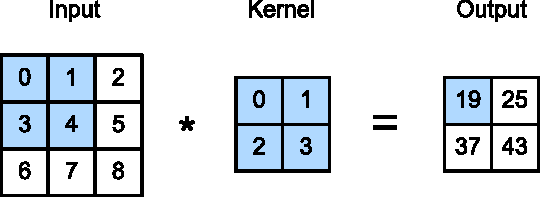
\includegraphics{../graph-visuals/convolution-example.pdf}
	\caption{Primer operacije konvolucije kernela ($2 \times 2$) sa slikom $(3 \times 3)$ sa korakom 1}
\end{figure}\\
Konvolucioni sloj sačinjen je od nekoliko \textit{filtera} / kernela (matrica realnih brojeva) koji su najčešće malih dimenzija ($2\times 2,3 \times 3,5 \times 5$,...).
Da bi se dobio izlaz konvolucionog sloja za svaki filter se računa operacija \textit{konvolucije}, odnosno matematički ispravnije
kros-korelacija filtera i ulazne slike.
\begin{figure}[!ht]
	\centering
    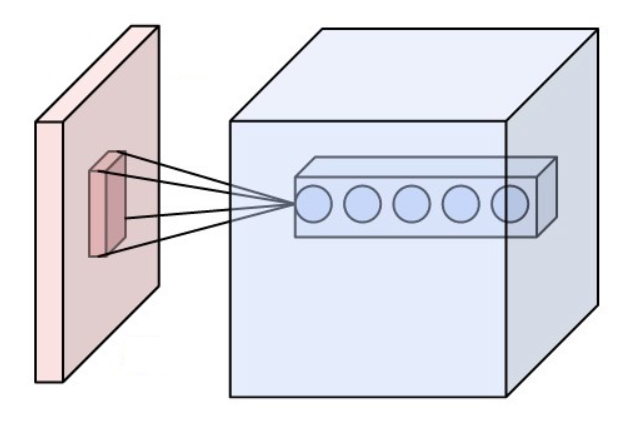
\includegraphics[scale=0.4]{../graph-visuals/conv-filter.png}
	\caption{Primer konvolucionog sloja}
\end{figure}\\
Najčešće ulazna slika ima dubinu veću od 1. Pa se najčešće za jedan filter računa konvolucija sa čitavom dubinom slike.
Na primer ako je ulazna slika dimenzije $(100 \times 100 \times 3)$ ako se uzme filter $(5 \times 5)$ za konvoluciju bio bi 
dubine takođe 3. Tj. dimenzija $(5 \times 5 \times 3)$. Takođe konvolucioni sloj ima nekoliko različitih filtera pa se za svaki od
filtera računaju konvolucije, time se dobija dubina u izlazu tog sloja (na primer na slici iznad ima 5 filtera pa je izlaz dubine 5).
Konvolucioni sloj takođe određuje veličina koraka (tj. \textit{stride}). Stride predstavlja za koliko se filter pomeri prilikom računanja
proizvoda sa ulaznom slikom. 
\begin{figure}[!ht]
	\centering
    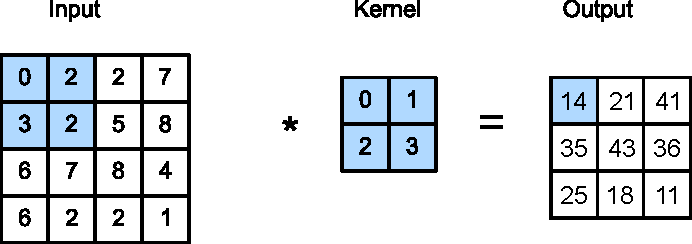
\includegraphics[scale=1]{../graph-visuals/convolution-operation-stride-1.pdf}
	\caption{Primer konvolucije slike $(4 \times 4 \times 1)$ sa filterom $(2 \times 2)$ sa korakom 1}
\end{figure}\\
\begin{figure}[!ht]
	\centering
    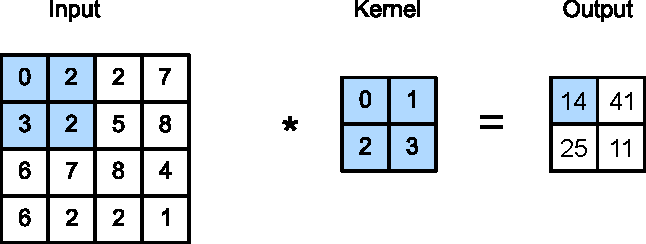
\includegraphics[scale=1]{../graph-visuals/convolution-operation-stride-2.pdf}
	\caption{Primer konvolucije slike $(4 \times 4 \times 1)$ sa filterom $(2 \times 2)$ sa korakom 2}
\end{figure}\\
Veličina filtera, broj filtera i korak definišu jedan konvolucioni sloj. Takođe, nakon računanja konvolucije
vrednosti iz rezultujuće matrice se prosleđuju u aktivacionu funkciju, najčešće ReLU. Pored konvolucionih slojeva koriste se
i takozvani \textit{pooling} slojevi.
\begin{figure}[!ht]
	\centering
    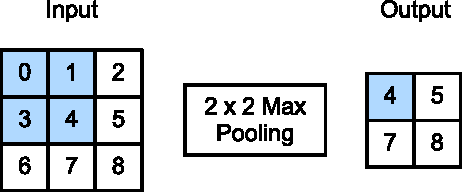
\includegraphics[scale=1]{../graph-visuals/max-pooling.pdf}
	\caption{Primer max pooling sloja sa dimenzijom $(2 \times 2)$}
\end{figure}\\
Pooling slojevi računaju neku funkciju (najčešće maksimum ili prosek) na nekom malom delu slike određenom pomoću veličine kernela,
slično kao i konvolucija. Cilj pooling slojeva je da smanje dimenzionalnost ulazne slike. Izlazi poslednjeg pooling sloja se
izravnjaju u vektor koji se zatim prosleđuje u jedan ili više potpuno povezanih slojeva, kako bi se na kraju dobio izlazni vektor
odgovarajuće dimenzije. Kako konvolucioni slojevi vrše diferencijabilne operacije jasno je da se i na ovakve neuronske mreže mogu
primeniti algoritmi zasnovani na određivanju gradijenta.
\section{Deep Q-learning}
Kada je broj mogućih stanja u nekom markovljevom procesu previše velik nalaženje $Q$ vrednosti za svaki par stanja i akcije je praktično
nemoguće. Na primer ako treba rešiti igru koja je predstavljena igraču grafički, poput većine video igara ili jednostavnije -
arkadnih Atari igara, stanje je cela slika koja je predstavljena igraču. Na primer za Atari igre slika je dimenzija $(160 \times 192)$
i postoji 128 mogućih boja. Pa je broj stanja ograničen odozgo sa $128^{160\cdot 192}$ što je očigledno previše velik broj stanja da bi
se uopšte čuvao u memoriji.\\
Međutim, pretpostavka koja ipak omogućava da agent nauči optimalnu politiku je da iako su stanja visoko dimenziona količina informacija je
prilično ograničena. Na primer verovatno je dovoljno znati da se na ekranu nalaze dva neprijatelja na određenoj udaljenosti kako bi
se igralo optimalno. Pa je nada da ukoliko se koristi model sposoban da dovoljno apstrakuje stanja da će takav model moći da
prepozna slična stanja i izgradi optimalnu politiku nad samo neophodnim informacijama. Međutim, aproksimacija $Q$ funkcije pomoću
nelinearnog modela je težak problem koji je tek skorije u nekoj meri rešen. Poznate su situacije gde nelinearni aproksimatori
$Q$ funkcije ne konvergiraju na optimalnu $Q$ vrednost, šta više čak i divergiraju u potpunosti (\latin \cite{NEURIPS2018_5fd0245f}). 
Međutim ukoliko se $Q$ funkcija aproksimira neuronskom mrežom i treniranje se vrši na specifičan način u praksi je često moguće dobiti
veoma dobre rezultate.\\
Kako bi se aproksimirala $Q$ funkcija posmatrajmo jednačinu za stohastičku verziju nalaženja optimalne $Q$ vrednosti:\\
Ako je data epizoda: $E: s_0,a_0,r_0,s_1,a_1,r_1,...,s_n,a_n,r_n$\\
Onda je u iteraciji $n$, za svako $s$ i svako $a$:\\
\[ 
	Q_n(s,a) =
	\begin{cases}
		(1-\alpha_n)Q_{n-1}(s,a) + \alpha_n (r_n + \gamma \text{max}_{a'}Q_{n-1}(s',a')), & \text{ako } s_n = s, a_n = a\\
		Q_{n-1}(s,a), & \text{u suprotnom}
	\end{cases}
\]
Ili u alternativnoj, ekvivalentnoj formulaciji:
\[ 
	Q_n(s,a) =
	\begin{cases}
		Q_{n-1}(s,a) + \alpha_n (r_n + \gamma \text{max}_{a'}Q_{n-1}(s',a') - Q_{n-1}(s,a)), & \text{ako } s_n = s, a_n = a\\
		Q_{n-1}(s,a), & \text{u suprotnom}
	\end{cases}
\]
Vrednost $r_n + \gamma \text{max}_{a'}Q_{n-1}(s',a') - Q_{n-1}(s,a)$ naziva se TD-greška (temporal difference error). Ako se ovo
posmatra kao vrednost koju treba minimizovati može se upotrebiti neuronska mreža na sledeći način:
Preformulišimo $Q$ funkciju kao neuronsku mrežu, sa parametrima $\theta$ odnosno $Q(s,a,\theta)$. Pa je TD greška ekvivalentna:
\[L_n(\theta_n) = (r_n + \gamma \text{max}_{a'}Q_{n-1}(s'_n,a',\theta_{n-1}) - Q_{n-1}(s_n,a_n,\theta_n))^2 \]
Učenje teče isto kao i za normalne neuronske mreže tako što se za svaki uzorak $(s_n,a_n,r_n,s_n')$ parametri mreže menjaju na sledeći način:
\[ \theta_n = \theta_{n-1} - \eta  \nabla L_n(\theta_{n-1}) \]
\medskip\\
Ovako formulisano učenje međutim nije preterano uspešno. Ako se učenje posmatra kao regresija i vrednost $r_n + \gamma \text{max}_{a'}Q_{n-1}(s'_n,a',\theta_{n-1})$ 
kao vrednost koju treba predvideti vidi se da se premenljiva koju treba predvideti veoma često menja što destabilizuje učenje, takođe
pokazano je da ovakav način učenja često precenjuje vrednost nagrade (\latin \cite{van2016deep}) pa
se u praksi fiksiraju dva seta paramatara $\theta$ i $\theta'$. Pa se funkcija gubitka definiše kao:
\[L_n(\theta_n) = (r_n + \gamma \text{max}_{a'}Q_{n-1}(s'_n,a',\theta) - Q_{n-1}(s_n,a_n,\theta_n'))^2 \]
Pa se na neki fiksan broj koraka razmenjuju mesta mrežama $\theta$ i $\theta'$.
Takođe moguće je i formulisati funkciju gubitka na sledeći način kako bi se izbeglo precenjivanje nagrade:
\[L_n(\theta_n) = (r_n + \gamma Q(s',\text{argmax}_{a'}Q_{n-1}(s'_n,a',\theta),\theta_n') - Q_{n-1}(s_n,a_n,\theta_n'))^2 \]
Ovo se naziva \textit{Double DQN} (\latin \cite{van2016deep}).
Pored ovih tehnika, primećeno je da kada se neuronske mreže koriste za aproksimaciju $Q$ funkcije, često dolazi do divergencije ili
lošeg učenja zbog velike korelacije među $Q$ vrednostima ako četvorke $(s,a,s',r)$ predstavljaju uzastopne četvorke neke epizode.
Kako bi se izbegla korelacija četvorke iskustva $(s,a,s',r)$ koje mreža generiše prilikom interakcije sa okruženjem dodaju se 
u velik niz iskustava odakle se prilikom treniranja biraju nasumične četvorke $(s,a,s',r)$ na kojima se mreža trenira. Ovo se naziva
\textit{experience replay} (\latin \cite{mnih2015human}).
\renewcommand\bibname{ Literatura}
 \addcontentsline{toc}{chapter}{ Literatura}
\latin
\printbibliography[title=Literatura]
\medskip


\end{document}
